\documentclass[a4paper,8pt]{article}

% Encoding.
\usepackage{geometry}
\usepackage[T2A]{fontenc}
\usepackage[utf8]{inputenc}
\usepackage[english,russian]{babel}

% Code insertion.
\usepackage[outputdir=build]{minted}

% Math functions.
\usepackage{amsmath}

% Image insertion.
\usepackage{svg}

% No line breaks.
\usepackage[none]{hyphenat}

\title{Задание 2: классификатор изображений}
\author{
         Смирнов Александр 
}

\date{\today}

\begin{document}

\maketitle

\section*{Обзор}


    \begin{figure}[h]
        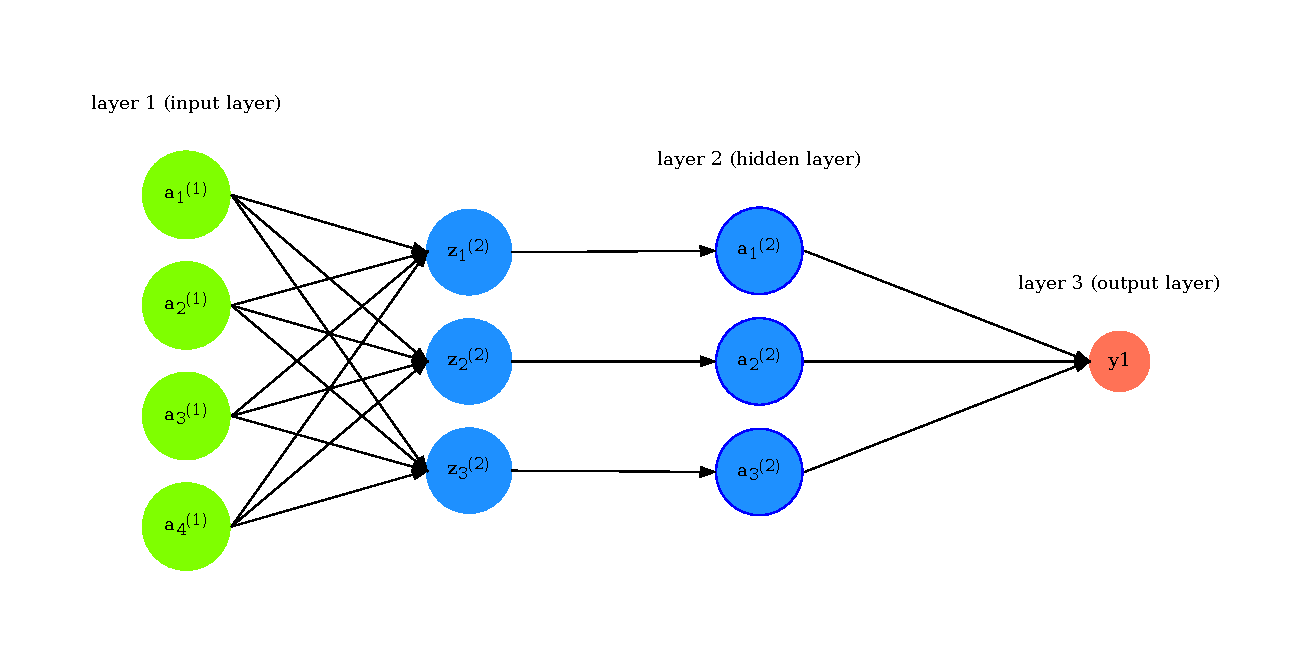
\includegraphics[width=0.9\textwidth]{./pic/architecture.pdf}
        \centering
    \end{figure}

Трёхслойная нейронная сеть состоит из четырех нейронов входного слоя, трёх нейронов на скрытом слое и 1 нейрона на выходном слое.

Нейроны зелёного цвета представляют собой входные данные:

\begin{itemize}
    \item 0: чёрный;
    \item 1: серый;
    \item 2: белый.
\end{itemize}

Первый набор активаций равен входным значениям. ``Активация'' -- значение нейрона после применения функции активации.




\end{document}
